\section{Radio Astronomy}\label{ra}
%--------------------------------------------------------------------------------------
\subsection{Radio Telescopes}\label{ra:sec:rt}
%
\subsubsection{Radio Telescope Design}
The most common design for radio telescopes is that of the parabolic reflector antenna. The design is a large parabolic dish with a sub-reflector at the parabola's focal point channeling the input into the feed horn at the center of the dish, a diagram of this can be seen in Figure \ref{ra:fig:para}. While it is possible to have a single antenna as a telescope for radio astronomy, in order for them to produce meaningful results, the antenna need to be extremely large (diameter of $+70$m) which in most cases can be structurally infeasible especially if the antenna is made to be steerable. Instead, a series of smaller ($8\sim30$m) antenna are used collectively in an array to produce a more accurate signal detection. These arrays do so through radio interferometry \citep{cheng2009radio}.
%
\begin{figure}[H]
	\centering
	%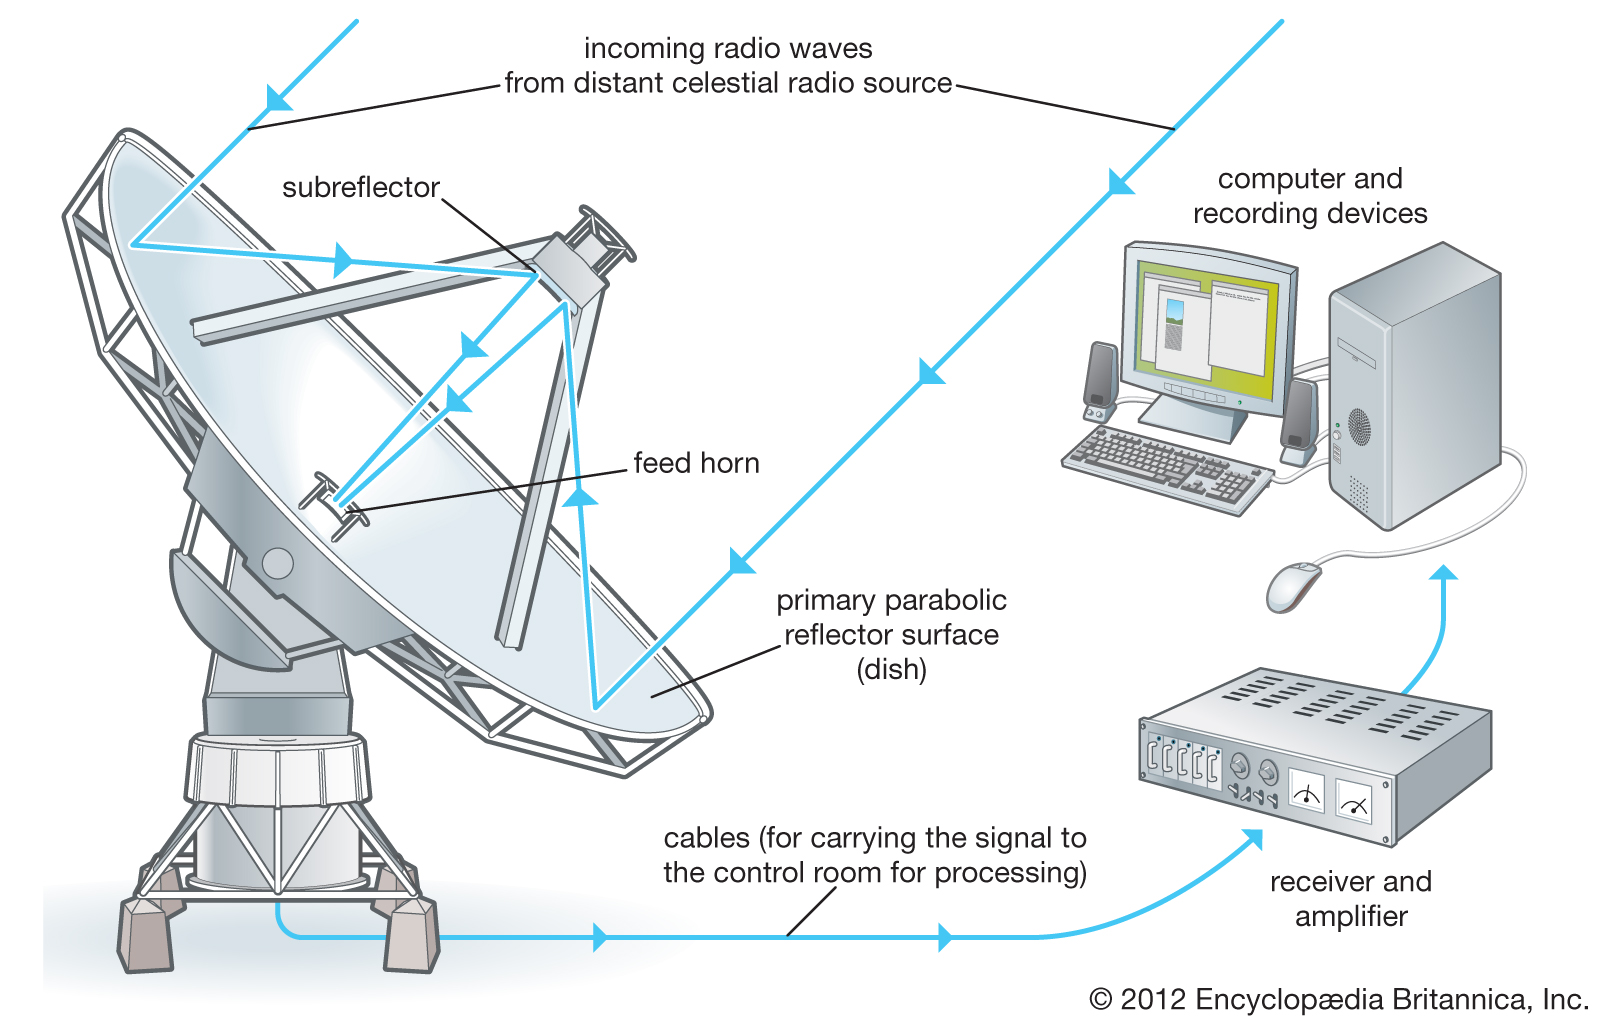
\includegraphics[width=0.5\textwidth]{Images/Telescope.jpg}
	\caption{Parabolic Reflector Antenna Design \citep{telescope}}
	\label{ra:fig:para}
\end{figure}
%
\subsubsection{Radio Interferometry}\label{ra:ssec:des}
Radio Interferometry uses an array of antennas to detect and measure objects emitting radiation in the radio-wave frequencies. Radio waves are defined as electromagnetic radiation with wavelengths of the order of $10^{-3}$ to $10^5$ meters \citep{cheng2009radio}. The interferometers finds the source of these waves by detecting minor delays in the parallel ray signal transmitted by the radiating source (source) as well as the amplitude and frequency of the source to calculate the position, size and intensity of the source \citep{thompson2008interferometry}.
%
\subsubsection{The SKA}
The SKA project was launched in order to create the world's largest array of radio telescopes. This will be achieved by having 197 radio telescopes situated in South Africa and Australia working together and having antenna thats' area will cover close to one square kilometer. The array is set to have a resolution of over 50 times that of the Hubble Space Telescope while still covering more massive areas of the sky (\cite{SKAsite}).
%--------------------------------------------------------------------------------------
\subsection{Image Capturing and Processing}\label{ra:sec:ic}
%
\subsubsection{The Primary Beam}\label{ra:ssec:tpb}
The primary beam is a mathematical function that describes the sensitivity pattern of an antenna. Naturally the beam is most sensitive in the center of the direction in which it is facing, with fringes of sensitivity radiating out as can be seen in Figure \ref{ra:fig:beam}. The circular sensitivity present in Figure \ref{ra:fig:beam} is also due to the fact that the telescope rotates in order to keep the center of the beam focused on the same area of the sky \citep{oleg}.
%
\begin{figure}[H]
	\centering
	%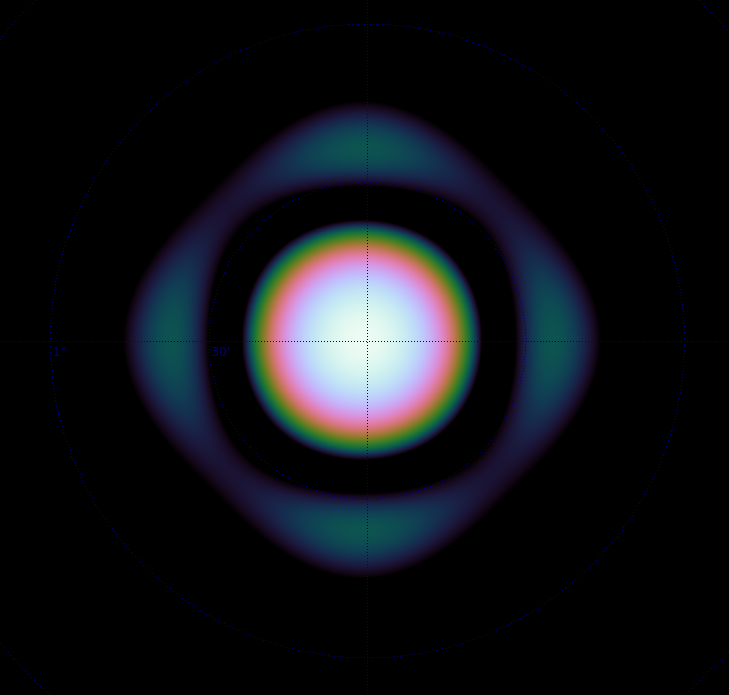
\includegraphics[scale=0.28]{Images/beam.png}
	\caption{Primary Beam Focus Pattern \citep{oleg}}
	\label{ra:fig:beam}
\end{figure}
%
\subsubsection{Aperture Synthesis}\label{ra:ssec:rii}
The electromagnetic radiation collected by the antenna is converted into voltage differences. The data is collected and stored over time (usually $\sim12$h) and the resulting phase differences in the data taken in by each antenna in the telescope is Fourier transformed from the frequency domain to that of the spatial domain, to give a two dimensional image \citep{sault1994multi}.
%
\subsubsection{Errors and Error Correcting}\label{ra:ssec:eec}
As with any real-world data input, the image capturing process of radio interferometry is subject to errors. These errors can be classified as arising from two main groups, namely Direction-independent (DI) and direction-dependent (DD) effects \citep{smirnov2015radio}. The DD-effects in particular arise from distortions due to interference from the ionosphere and deviations of the primary beam from the model. This distortion, $D$, can be corrected, but only relative to a chosen point, $\xi$. The correction at any given point, $E_i$, is dependent on the intensity at the point, $\boldsymbol{S}_i$, and the distortion at the point relative to $\xi$, $D(\boldsymbol{x}_i,\xi)$. It is important to note that the point-wise error is lowest at $\xi$, but any source at $\xi$ will radiate out with $D$ over the domain. It can therefore be seen that to minimize this error, every point can be made a correction seed and the image can be broken up by these points and reassembled to form an image with little to no error. However, this is computationally ineffective as there are hundreds of sources per image and also due to the fact that the image is sparely populated. We therefore seek a method which optimally compromises computational feasibility and error reduction \citep{oleg}.
%--------------------------------------------------------------------------------------
\subsection{Related Work: Naive Method}
The most basic compromise is dividing the image evenly into a grid of smaller images and correcting for these from either the center of the sub-image, the point with the strongest source or the ``center of mass'' (average location of points) of all the points in the sub-image, either weighted by intensity or not. The problem with this method lies in the fact that either the sub-image is void and has no definite points, if $\xi$ is set at the center, it could be far from every other point and has no substantial effect on reducing the overall error or if $\xi$ is set at the strongest source or the center of mass, it could lie too close to the boundary of the sub-image and, again, have no overall impact on error reduction \cite{oleg}.
%--------------------------------------------------------------------------------------



